% Created 2022-05-11 mer. 10:53
% Intended LaTeX compiler: pdflatex
\documentclass[11pt]{article}
\usepackage[utf8]{inputenc}
\usepackage[T1]{fontenc}
\usepackage{graphicx}
\usepackage{grffile}
\usepackage{longtable}
\usepackage{wrapfig}
\usepackage{rotating}
\usepackage[normalem]{ulem}
\usepackage{amsmath}
\usepackage{textcomp}
\usepackage{amssymb}
\usepackage{capt-of}
\usepackage{hyperref}
\usepackage{lmodern} % Ensures we have the right font
\usepackage{graphicx}
\usepackage{amsmath, amsthm, amssymb}
\usepackage[table, xcdraw]{xcolor}
\usepackage{fancyhdr}
\usepackage[left=2cm,right=2cm,top=3cm,bottom=3cm]{geometry}
\pagestyle{fancy}
\fancyhf{}
\lhead{Modify in current org file : \lhead{foo}}
\rfoot{Page \thepage}
\usepackage{titling}
\setlength{\droptitle}{-8ex}
\pretitle{\begin{flushleft}\Large\bfseries}
\posttitle{\par\end{flushleft}}
\preauthor{\begin{flushleft}\large}
\postauthor{\end{flushleft}}
\predate{\begin{flushleft}}
\postdate{\end{flushleft}}
\usepackage[normalem]{ulem}
\usepackage{sectsty}
\sectionfont{\underline}
\makeatletter
\def\@seccntformat#1{%
\expandafter\ifx\csname c@#1\endcsname\c@section\else
\csname the#1\endcsname\quad
\fi}
\makeatother
\definecolor{bblue}{HTML}{275382}
\usepackage[colorlinks]{hyperref}
\hypersetup{colorlinks, linkcolor=bblue, urlcolor=bblue}
\usepackage[font={color=gray},figurename=Fig.,labelfont={it}]{caption}
\setlength{\parindent}{0pt}
\usepackage{graphicx}
\setkeys{Gin}{width=0.8\linewidth}
\setkeys{Gin}{height=0.7\textheight}
\setkeys{Gin}{keepaspectratio}
\usepackage{enumitem}
\setlist{noitemsep}
\setlist[itemize]{noitemsep}
\renewcommand{\contentsname}{Sommaire}
\usepackage{listings}
\usepackage{xcolor}
\usepackage[utf8]{inputenc}
\usepackage[table]{color}
\definecolor{grayW}{rgb}{0.94,0.94,1.00}
\definecolor{bluegr}{rgb}{0.0,0.50,0.50}
\definecolor{redp}{rgb}{0.80,0.10,0.10}
\lstset{
backgroundcolor=\color{grayW},
keywordstyle=\color{bluegr},
stringstyle=\color{redp},
basicstyle=\ttfamily\scriptsize,
breakatwhitespace=false,
numbers=left,
numbersep=5pt,
}
\lhead{DUREL Enzo, VILLEPREUX Thibault}
\rhead{Serveur Web}
\author{DUREL Enzo, VILLEPREUX Thibault}
\date{\today}
\title{Serveur Web}
\hypersetup{
 pdfauthor={DUREL Enzo, VILLEPREUX Thibault},
 pdftitle={Serveur Web},
 pdfkeywords={},
 pdfsubject={},
 pdfcreator={Emacs 27.1 (Org mode 9.3)}, 
 pdflang={English}}
\begin{document}

\maketitle
\tableofcontents

\thispagestyle{fancy}

\newpage

\section{Introduction}
\label{sec:org40456fe}

Nous avons créé un serveur.

\section{Fonctionnalités importantes}
\label{sec:orgc280ad7}

\begin{quote}
Quelles sont les fonctionnalités qui vous semblent importantes ?
\end{quote}

L'objectif est de créer un dispositif où les élèves peuvent consulter leur carnet dématérialisé. Il faut également prévoir la possibilité à un professeur de mettre des gommettes à un élève.

Plus précisément, si le professeur est connecté il peut faire plusieurs actions :
\begin{itemize}
\item ajouter, supprimer ou modifier un élève (son nom et son prénom)
\item lister, ajouter ou supprimer une gommette attribuée à un élève. Une gommette attribuée possède une date, un motif et une gommette principale qui elle-même contient une couleur (rouge, vert ou blanc) et une description générale.
\item créer un nouveau professeur
\item se déconnecter de sa session
\end{itemize}

En revanche tout le monde a accès à la liste des gommettes configurées et la liste des gommettes de chaque élève, avec possibilité de voir le professeur ayant mis la gommette.

\section{Principales classes}
\label{sec:org756013a}

\begin{figure}[htbp]
\centering
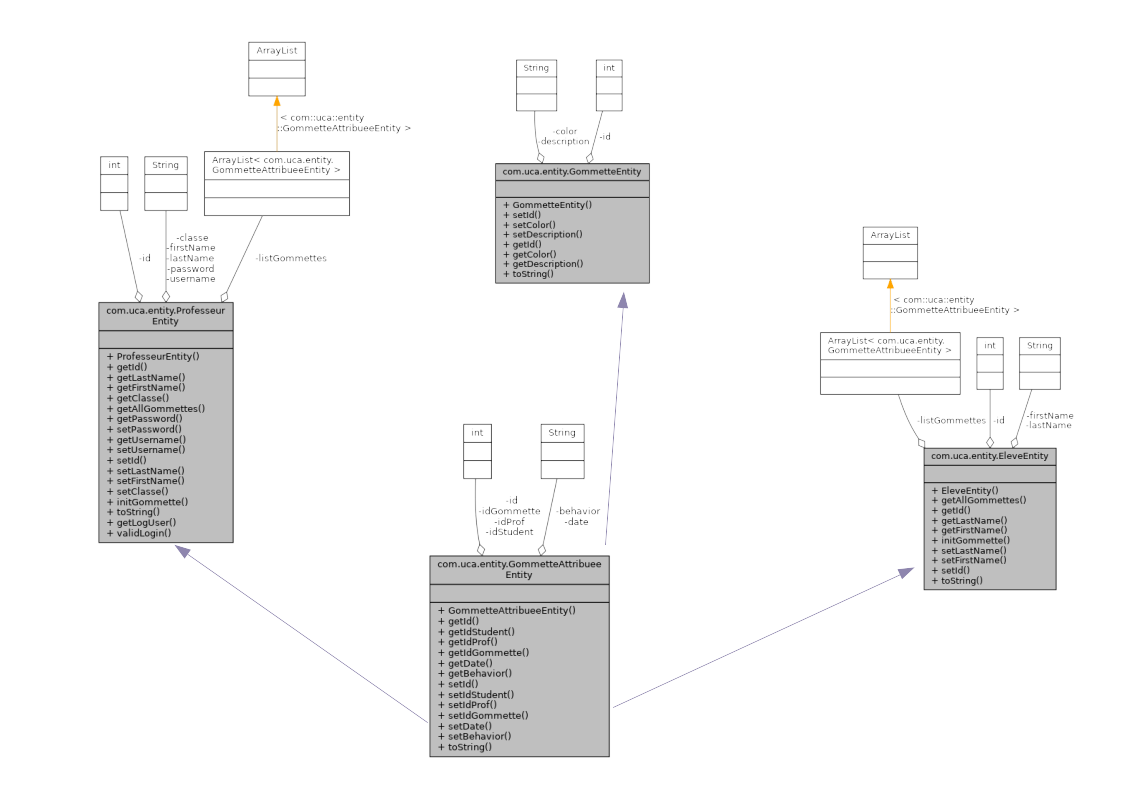
\includegraphics[width=.9\linewidth]{./uml.png}
\caption{UML des entités}
\end{figure}

Image disponible \href{./uml.png}{ici} (./web-server/rapport/uml.png)

\begin{quote}
Quelles vont être les principales classes de votre applications ?
\end{quote}

\section{Bases de données}
\label{sec:org80b80d1}

\begin{quote}
Quelles vont être les tables de votre base de données ?
\end{quote}

Chaque classe principale possède une table dans la base de donnée relationnelle. 

La table "PROFESSEURS" comme son nom l'indique représente la classe ProfesseurEntity, voici sa représentation avec quelques exemples :


\begin{center}
\begin{tabular}{rllll}
Id (INT, primary key) & Firstname ( VARCHAR 100) & Lastname (VARCHAR 100) & Usrename (VARCHAR  100) & Password (VARCHAR 100)\\
\hline
1 & Paul & Boulanger & paboulanger & password\\
2 & Jules & Verne & juverne & azerty1234\\
3 & Georges & Lefou & gelefou & 123456789\\
\end{tabular}
\end{center}


La table "ELEVES" comme son nom l'indique représente la classe EleveEntity, voici sa représentation avec quelques exemples :

\begin{center}
\begin{tabular}{rll}
Id (INT, primary key) & Firstname ( VARCHAR 100) & Lastname (VARCHAR 100)\\
\hline
1 & Jean & Valjean\\
2 & Thomas & Ducarquoi\\
3 & Timothée & Louis\\
\end{tabular}
\end{center}


La table "GOMMETTES" comme son nom l'indique représente la classe GommetteEntity, voici sa représentation avec quelques exemples :

\begin{center}
\begin{tabular}{rll}
Id (INT, primary key) & Color (VARCHAR 50) & Description (VARCHAR 100)\\
\hline
1 & Rouge & Bavardage\\
2 & Vert & Excellente note\\
3 & Blanc & Nettoie les toilettes\\
\end{tabular}
\end{center}


La table "GOMMETTESATTRIBUEES" comme son nom l'indique représente la classe GommetteAttribueeEntity, voici sa représentation avec quelques exemples :

\begin{center}
\begin{tabular}{rrrrrl}
Id (INT, primary key) & Id\textsubscript{student} (INT) & Id\textsubscript{prof} (INT) & Id\textsubscript{gommette} (INT) & Date (VARCHAR 100) & Behavior (VACHAR 10\textsubscript{000})\\
\hline
1 & 1 & 1 & 2 & 2022-02-09 & Jette de la nourriture sur son camarade\\
2 & 2 & 1 & 1 & 2022-06-07 & A fait tous ces devoirs sans erreurs\\
2 & 3 & 1 & 3 & 2022-04-07 & Aide son camarade à faire ces lacets\\
\end{tabular}
\end{center}


La date est en format VARCHAR. En effet, nous avons un formulaire HTML avec comme type une "date" afin de faciliter la saisie de date pour l'utilisateur grâce à l'apartirion d'un "calendrier dynamique". Cette date est en réalité une chaîne de caractère, ce qui nous arrange bien afin de la stockée dans la base de donnée.
\section{Technologies utilisées}
\label{sec:org7289004}
\begin{quote}
Quelles solutions technologiques envisagez-vous ?
\end{quote}

\section{Routes}
\label{sec:org7dacbae}
\subsection{login}
\label{sec:org8bdbe68}
\subsubsection{login}
\label{sec:org9b51c1a}

\begin{quote}
GET "\url{http://localhost:8081/login}"
\end{quote}

Page de connexion qui sert aussi de page principale au site.

\begin{quote}
POST "\url{http://localhost:8081/login}"
\end{quote}

Méthode de vérification des identifiants du professeur, renvoie sur l'ent du professeur en cas 
de succes.

\subsubsection{logout}
\label{sec:orgaa564a5}

\begin{quote}
GET "\url{http://localhost:8081/logout}"
\end{quote}

Méthode de déconnexion, redirige sur le login après la suppression de la session
et du cookie de connexion.

\subsection{eleves}
\label{sec:org5190c36}

\begin{quote}
GET "\url{http://localhost:8081/eleves}"
\end{quote}

Affiche la liste des élèves avec leur gommette attribuées.

\subsubsection{eleve}
\label{sec:orgf405e2d}

\begin{quote}
GET "\url{http://localhost:8081/eleves/:id}"
\end{quote}

Affiche la page de profil de l'élève (nom, prénom, liste des gommettes attribuées).

\subsubsection{create}
\label{sec:org35c327a}

\begin{quote}
GET "\url{http://localhost:8081/eleves/create}"
\end{quote}

Affiche la page de création d'un élève (formulaire).

\begin{quote}
POST "\url{http://localhost:8081/eleves/create}"
\end{quote}

Création de l'élève dans la bdd. Un élève est représenté par son nom et son prénom.

\subsubsection{delete}
\label{sec:org7ca64c8}

\begin{quote}
GET "\url{http://localhost:8081/eleves/delete:id}"
\end{quote}

Méthode de suppression d'un élève dont l'id dans l'uri correspond à l'id de l'élève dans la bdd.
redirige vers la liste d'élèves.

\subsubsection{modify}
\label{sec:org562fc68}

\begin{quote}
GET "\url{http://localhost:8081/eleves/modify/:id}"
\end{quote}

Méthode de suppression d'un élève dont l'id dans l'uri correspond à l'id de l'élève dans la bdd.

\begin{quote}
POST "\url{http://localhost:8081/eleves/modify/:id}"
\end{quote}

Modification de l'élève dans la bdd. L'id est spécifié dans l'uri.

\subsection{professeurs}
\label{sec:org3685dee}
\subsubsection{professeur}
\label{sec:org83091d6}

\begin{quote}
GET "\url{http://localhost:8081/professeurs/:id}"
\end{quote}

Affiche la page personnelle du professeur. Elle sert de page d'accueil et d'ent au professeur.
Elle possède les interaction de base telle que création d'un élève, création d'une gommette,
attribution d'une gommette à un élève.

\subsubsection{create}
\label{sec:org686ea93}

\begin{quote}
GET "\url{http://localhost:8081/professeurs/create}"
\end{quote}

Affiche la page de création d'un professeur. Un professeur est représenté par : nom, prénom, nom d'utilisateur, mot de passe.

\begin{quote}
POST "\url{http://localhost:8081/professeurs/create}"
\end{quote}

Création du professeur dans la bdd.

\subsubsection{delete}
\label{sec:org155f98a}

\begin{quote}
GET "\url{http://localhost:8081/professeurs/delete/:id}"
\end{quote}

Création d'un professeur en bdd.

\subsection{gommettes}
\label{sec:org70398c3}

\begin{quote}
GET "\url{http://localhost:8081/gommettes}"
\end{quote}

Affiche la page de la liste des gommettes.

\subsubsection{create}
\label{sec:org1a91f5b}

\begin{quote}
GET "\url{http://localhost:8081/gommettes/create}"
\end{quote}

Affiche la page de création des gommettes.

\begin{quote}
POST "\url{http://localhost:8081/gommettes/create}"
\end{quote}

Création de la gommette en bdd.

\subsubsection{delete}
\label{sec:org488da5f}

\begin{quote}
GET "\url{http://localhost:8081/gommettes/delete:id}"
\end{quote}

Méthode de suppression de la gommette, redirige vers la page de la liste des gommettes.

\subsubsection{modify}
\label{sec:org9b9f074}

\begin{quote}
GET "\url{http://localhost:8081/gommettes/modify/:id}"
\end{quote}

Méthode de suppression d'une gommette dont l'id dans l'uri correspond à l'id de la gommette dans la bdd.

\begin{quote}
POST "\url{http://localhost:8081/eleves/modify/:id}"
\end{quote}

Modification de la gommette dans la bdd. L'id est spécifié dans l'uri.

\subsubsection{attribuees}
\label{sec:orgc12268c}
\begin{enumerate}
\item create
\label{sec:org09997f7}

\begin{quote}
GET "\url{http://localhost:8081/gommettes/attribuees/create/:id}"
\end{quote}

Affiche la page d'attribution d'une gommette pour l'élève dont l'id est spécifiée dans l'uri.

\begin{quote}
POST "\url{http://localhost:8081/gommettes/attribuees/create/:id}"
\end{quote}

Création de la gommette attribuee en bdd.

\item delete
\label{sec:org59dafab}

\begin{quote}
GET "\url{http://localhost:8081/gommettes/attribuees/delete/:id}"
\end{quote}

Méthode de suppression de la gommette\textsubscript{attribuee}, l'id correspond à celui de l'élève à qui 
la gommette a été attribuée.

\newpage
\listoffigures
\end{enumerate}
\end{document}
